%%
%% This is file `sample-sigconf.tex',
%% generated with the docstrip utility.
%%
%% The original source files were:
%%
%% samples.dtx  (with options: `all,proceedings,bibtex,sigconf')
%% 
%% IMPORTANT NOTICE:
%% 
%% For the copyright see the source file.
%% 
%% Any modified versions of this file must be renamed
%% with new filenames distinct from sample-sigconf.tex.
%% 
%% For distribution of the original source see the terms
%% for copying and modification in the file samples.dtx.
%% 
%% This generated file may be distributed as long as the
%% original source files, as listed above, are part of the
%% same distribution. (The sources need not necessarily be
%% in the same archive or directory.)
%%
%%
%% Commands for TeXCount
%TC:macro \cite [option:text,text]
%TC:macro \citep [option:text,text]
%TC:macro \citet [option:text,text]
%TC:envir table 0 1
%TC:envir table* 0 1
%TC:envir tabular [ignore] word
%TC:envir displaymath 0 word
%TC:envir math 0 word
%TC:envir comment 0 0
%%
%% The first command in your LaTeX source must be the \documentclass
%% command.
%%
%% For submission and review of your manuscript please change the
%% command to \documentclass[manuscript, screen, review]{acmart}.
%%
%% When submitting camera ready or to TAPS, please change the command
%% to \documentclass[sigconf]{acmart} or whichever template is required
%% for your publication.
%%
%%
\documentclass[sigconf]{acmart}
\usepackage{caption}
\usepackage{subcaption}
%%
%% \BibTeX command to typeset BibTeX logo in the docs
\AtBeginDocument{%
  \providecommand\BibTeX{{%
    Bib\TeX}}}

%% Rights management information.  This information is sent to you
%% when you complete the rights form.  These commands have SAMPLE
%% values in them; it is your responsibility as an author to replace
%% the commands and values with those provided to you when you
%% complete the rights form.
\setcopyright{acmlicensed}
\copyrightyear{2026}
\acmYear{2026}
\setcopyright{cc}
\setcctype{by-nc-nd}
\acmConference[SIGGRAPH Talks '26]{Special Interest Group on Computer Graphics and Interactive Techniques Conference Talks}{July 19--23, 2026}{Los Angeles, CA, USA}
\acmBooktitle{Special Interest Group on Computer Graphics and Interactive Techniques Conference Talks (SIGGRAPH Talks '26), July 19--23, 2026, Los Angeles, CA, USA}
\acmDOI{10.1145/3799818.3812087}
\acmISBN{979-8-4007-2541-8/2026/07}

%%
%%  Uncomment \acmBooktitle if the title of the proceedings is different
%%  from ``Proceedings of ...''!
%%
%%\acmBooktitle{Woodstock '18: ACM Symposium on Neural Gaze Detection,
%%  June 03--05, 2018, Woodstock, NY}
\acmISBN{978-1-4503-XXXX-X/2026/07}

\usepackage{gensymb}
%%
%% Submission ID.
%% Use this when submitting an article to a sponsored event. You'll
%% receive a unique submission ID from the organizers
%% of the event, and this ID should be used as the parameter to this command.
%%\acmSubmissionID{123-A56-BU3}

%%
%% For managing citations, it is recommended to use bibliography
%% files in BibTeX format.
%%
%% You can then either use BibTeX with the ACM-Reference-Format style,
%% or BibLaTeX with the acmnumeric or acmauthoryear sytles, that include
%% support for advanced citation of software artefact from the
%% biblatex-software package, also separately available on CTAN.
%%
%% Look at the sample-*-biblatex.tex files for templates showcasing
%% the biblatex styles.
%%

%%
%% The majority of ACM publications use numbered citations and
%% references.  The command \citestyle{authoryear} switches to the
%% "author year" style.
%%
%% If you are preparing content for an event
%% sponsored by ACM SIGGRAPH, you must use the "author year" style of
%% citations and references.
%% Uncommenting
%% the next command will enable that style.
\citestyle{acmauthoryear} 


%%
%% end of the preamble, start of the body of the document source.
\begin{document}

%%
%% The "title" command has an optional parameter,
%% allowing the author to define a "short title" to be used in page headers.
\title{In Defense of Euler Angles in Game Programming}

%%
%% The "author" command and its associated commands are used to define
%% the authors and their affiliations.
%% Of note is the shared affiliation of the first two authors, and the
%% "authornote" and "authornotemark" commands
%% used to denote shared contribution to the research.
\author{Matthew Whiting}
\affiliation{%
  \institution{University of Southern California}
  \city{Los Angeles}
  \state{California}
  \country{USA}}
\email{whitingm@usc.edu}

%%
%% The abstract is a short summary of the work to be presented in the
%% article.
\begin{abstract}
When teaching three-dimensional rotations, instruction often moves quickly from Euler angles to quaternions. This is even the approach in our Video Game Programming course at the University of Southern California. The prevailing rationale repeated by both educators and those in industry is that we avoid Euler angles due to gimbal lock and the associated loss of a degree of freedom. However, an analysis of the typical problems in game development shows that in most cases, we do not actually need three degrees of freedom. Thus, in many cases Euler angles can be a simpler, more convenient approach than quaternions. In fact, many typical rotational problems in games are inherently constrained to two degrees of freedom. In these cases, quaternion interpolation (spherical linear interpolation or slerp) can produce undesirable effects, whereas Euler angle interpolation produces the desired result. Common examples include target tracking scenarios defined by azimuth and elevation (yaw and pitch), as well as camera systems in which player input is explicitly divided along these axes.
  
This paper argues that Euler angles should be presented as a first-class representation for constrained rotational problems. By teaching both Euler angles and quaternions as complementary tools, and by emphasizing practical techniques such as angle extraction using \textit{atan2}, educators can better equip students to select rotation representations that minimize complexity and produce predictable, application-appropriate motion.
\end{abstract}

%%
%% The code below is generated by the tool at http://dl.acm.org/ccs.cfm.
%% Please copy and paste the code instead of the example below.
%%
\begin{CCSXML}
<ccs2012>
   <concept>
       <concept_id>10010405.10010489</concept_id>
       <concept_desc>Applied computing~Education</concept_desc>
       <concept_significance>500</concept_significance>
       </concept>
   <concept>
       <concept_id>10010405.10010476.10011187.10011190</concept_id>
       <concept_desc>Applied computing~Computer games</concept_desc>
       <concept_significance>500</concept_significance>
       </concept>
   <concept>
       <concept_id>10003456.10003457.10003527.10003531.10003533</concept_id>
       <concept_desc>Social and professional topics~Computer science education</concept_desc>
       <concept_significance>300</concept_significance>
       </concept>
    <concept>
        <concept_id>10010147.10010371.10010352.10010378</concept_id>
        <concept_desc>Computing methodologies~Procedural animation</concept_desc>
        <concept_significance>300</concept_significance>
        </concept>
 </ccs2012>
\end{CCSXML}

\ccsdesc[500]{Applied computing~Education}
\ccsdesc[500]{Applied computing~Computer games}
\ccsdesc[300]{Social and professional topics~Computer science education}
\ccsdesc[300]{Computing methodologies~Procedural animation}

%%
%% Keywords. The author(s) should pick words that accurately describe
%% the work being presented. Separate the keywords with commas.
\keywords{Euler Angles, Quaternions, Gimbal Lock, Undergraduate Education, Game Programming, Altazimuth}

%%
%% This command processes the author and affiliation and title
%% information and builds the first part of the formatted document.
\maketitle

\section{Introduction}
When three-dimensional coordinate systems are first introduced, Euler angles are often presented as a natural and intuitive representation of orientation. As human beings, this is how we naturally navigate the world. For all practical purposes, we move around in the horizontal plane, turning left or right (yaw). When the need arises, we can look up or down (pitch), and although we are certainly capable of it, tilting sideways (roll) is rare in daily life.

In the context of three-dimensional graphics, however, instruction often shifts quickly toward quaternions. Euler angles are commonly characterized as problematic due to issues such as gimbal lock and poor interpolation behavior. As a result, quaternions are widely regarded as the superior and safer representation. This prevailing perspective has led many graphics and gameplay engineers to overlook scenarios in which Euler angles, by virtue of how they interpolate, may in fact be the more appropriate choice.

\section{Gimbal Lock}

The term \textit{gimbal lock} originates from physical mechanisms composed of concentric rotational frames, or gimbals. With three such rotational axes, a system can represent arbitrary orientation in three-dimensional space. However, at certain configurations, two of these axes may become aligned, reducing the system’s ability to distinguish rotations about those axes.

In practice, this alignment does not imply a true loss of rotational capability. For example, an aircraft oriented vertically still retains full control authority through its control surfaces and can execute pitch, roll, and yaw maneuvers in body space. The limitation instead arises in how those rotations are expressed relative to a fixed reference frame. 
%At low pitch angles, the ailerons of an aircraft primarily result in roll and the rudder produces yaw. But at \(90\degree\), the rudder will cause a change in pitch instead.
\begin{figure}[b]
     \centering
     \begin{subfigure}[b]{0.2\textwidth}
         \centering
         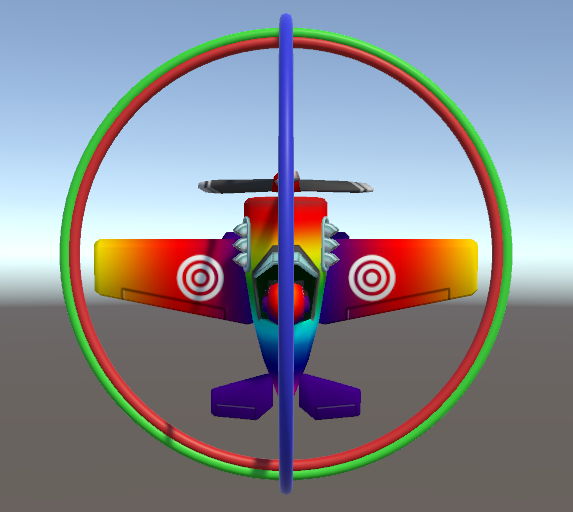
\includegraphics[width=\textwidth]{Gimbal01.png}
         \caption{Yaw And Roll Coincide}
%         \label{fig:gimbal01}
     \end{subfigure}
     \hfill
     \begin{subfigure}[b]{0.2\textwidth}
         \centering
         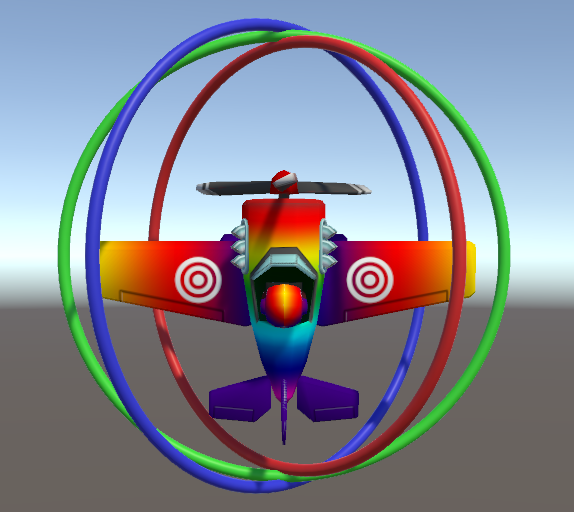
\includegraphics[width=\textwidth]{Gimbal02.png}
         \caption{Equivalent Orientation}
%         \label{fig:gimbal02}
     \end{subfigure}
    \caption{Gimbal Lock}
    \label{fig:gimbal}
\end{figure}
At a pitch of \(90\degree\), this alignment introduces a discontinuity in the Euler angle parameterization. This discontinuity is the source of the phenomenon commonly referred to as gimbal lock. (Figure \ref{fig:gimbal}) Importantly, in a computational context, Euler angles are a mathematical representation rather than a physical mechanism. There is no inherent constraint preventing the representation of arbitrary orientations, nor is any degree of rotational freedom lost. What is lost is the convenience of a smooth and continuous mapping between numeric parameters and spatial orientation.

While these discontinuities at the poles of the parameter space can be inconvenient, these singularities are an inherent characteristic in certain physical mechanical systems being modeled. In these cases, the singularity may not be resolved by switching to quaternions. Alternatively, there are practical approaches to resolve the singularity while relying primarily on Euler angle calculations. It is therefore necessary to consider the underlying rotational behavior being modeled and the constraints imposed by the chosen parameterization.

\section{Two Degrees of Freedom}
In many applications, the rotational behavior being modeled is inherently constrained to two degrees of freedom. A common example is a seated observer tracking a moving object within their field of view. While the object may move freely in three-dimensional space, the observer’s head motion can be described entirely by azimuth (rotation about the vertical axis or yaw) and elevation (rotation about the horizontal axis or pitch).
\begin{figure}[b]
     \centering
     \begin{subfigure}[b]{0.25\textwidth}
         \centering
         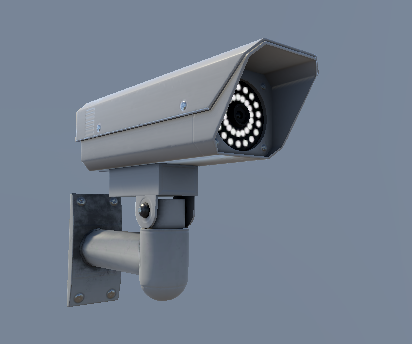
\includegraphics[width=\textwidth]{SecurityCamera.png}
         \caption{Camera with Altazimuth Mount}
         \label{fig:security camera}
     \end{subfigure}
     \hfill
     \begin{subfigure}[b]{0.25\textwidth}
         \centering
         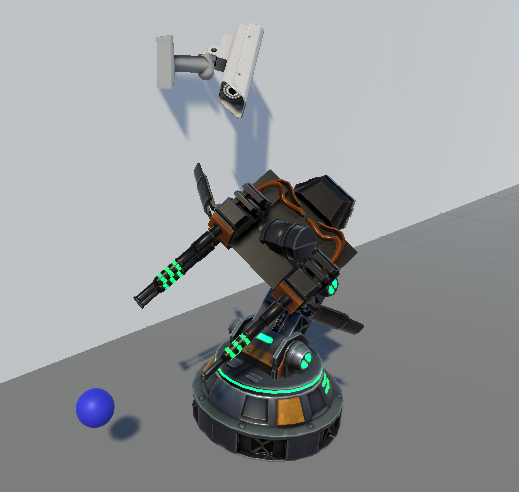
\includegraphics[width=\textwidth]{FlippedTurret.png}
         \caption{Turret Bending Over Backwards}
         \label{fig:turret}
     \end{subfigure}
    \label{fig:altazimuth}
    \caption{Two Degrees of Freedom}
\end{figure}
This azimuth–elevation representation is widely used in physical hardware, particularly for tasks involving target tracking or directional alignment. Camera systems, antenna arrays, and telescope mounts frequently employ so-called \textit{Az/El} or \textit{altazimuth} configurations (Figure \ref{fig:security camera}).

When such constrained motion is instead modeled using quaternions, unintended behavior can arise. For example, Figure \ref{fig:turret} illustrates a laser turret in a video game executing a spherical linear interpolation (slerp) between orientations in order to engage a target located behind it. While mathematically valid, this interpolation introduces rotational components that fall outside the intended azimuth–elevation constraint, producing motion that may be undesirable for the application.

\section{Video Game Camera}

Quaternions are frequently used by video game programmers to control virtual camera orientation \cite{Bobic}. While video games encompass a wide range of genres and camera systems, it is highly unusual for an in-game camera to intentionally rotate about the forward axis, commonly referred to as roll or \textit{Dutch tilt}.

Quaternion-based spherical linear interpolation (slerp) does not inherently respect this constraint. When orientations are interpolated freely in quaternion space, roll may be introduced even when it is not desired, requiring additional logic to suppress it. In contrast, Euler angle representations allow pitch, yaw, and roll to be interpolated independently, ensuring that interpolation between orientations does not introduce unintended roll.

In a typical third-person camera system, the camera orbits around a player-controlled avatar, and the player has two axes of input to guide the camera. Horizontal input commands the camera to orbit the avatar in the horizontal plane (yaw), while input on the forward axis produces pitch. These two inputs are intentionally decoupled. When a yaw rotation of \(180\degree\) is commanded, the expected behavior is a pure horizontal orbit with the pitch angle remaining unchanged. Quaternions are inherently more complex, and the resulting motion depends on what was expressed to create the quaternions. If the quaternion is generated as a shortest-path arc, slerp will traverse a great-circle arc over the poles while introducing unintended twist. Alternatively, a slerp between quaternions matching the equivalent Euler angles will be essentially indistinguishable from the Euler angle interpolation rendering the additional computational complexity completely unnecessary.
\begin{figure}[b]
     \centering
     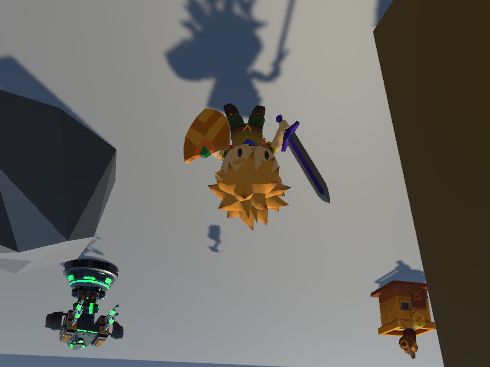
\includegraphics[width=0.8\linewidth]{CameraUpsideDown.png}
     \caption{Euler Angle Camera Crossing Poles Without Issue}
     \label{fig:Euler Camera}
\end{figure}
A common concern arises when an orbiting video game camera approaches a pitch of \(90\degree\): whether the camera will become “locked” due to a perceived loss of a degree of freedom (gimbal lock). Rather than lost freedom, in practice, the underlying issue is understanding the intention behind the user's control input. Once the desired mapping from two-dimensional input to camera motion is defined, it can be implemented directly - often in terms of Euler angles. Figure \ref{fig:Euler Camera} shows a third-person camera allowed to rotate past \(90\degree\) elevation using Euler angle calculations. This is not commonly allowed in video games, but it does not cause visual discontinuities or control issues.

\section{Animation}
While Euler angles can be effective in certain contexts, quaternions are generally preferred for jointed skeletal animation. Nevertheless, it is notable that Autodesk Maya defaults to Euler angles within its animation system \cite{Autodesk1}.

Euler angle interpolation operates in a decoupled manner, which can occasionally result in motion that appears unnatural. Additionally, interpolation near the poles of the parameter space can introduce discontinuities commonly associated with gimbal lock. In practice, however, skeletal joints are typically constrained to limited ranges of motion and seldom reach configurations in which these singularities occur. Consequently, artists are often able to work effectively using Euler angles without encountering significant issues.

Autodesk \cite{Autodesk1} acknowledges the limitations of Euler angle interpolation including gimbal lock and flipping (where interpolation from \(-180\degree\) to \(180\degree\) manifests as a \(360\degree\) rotation). However, they also point out the advantage that Euler angles can be made to rotate from \(0\degree\) to \(720\degree\) in a single pair of keyframes while there is no way to represent that type of motion using quaternions.

\section{atan2()}
It is also worth highlighting the role of the \textit{atan2} function in practical applications of Euler angles. Despite its convenience, this function is sometimes underutilized in graphics and game development workflows.

When converting Euler angles to position or direction vectors, the transformation is typically expressed using matrices composed of sine and cosine terms. Reversing this process might suggest the use of inverse sine and cosine functions; however, the inverse tangent function is often more practical. Most standard mathematics libraries provide a two-argument variant, \textit{atan2}, which resolves angular values correctly across all four quadrants.

Extracting a rotation angle from a two-dimensional vector is a common operation in video game programming as with the azimuth-tracking problems outlined previously. Traditional approaches may rely on the arc cosine of a normalized vector component combined with additional logic to determine the correct sign. The \textit{atan2} function provides a more direct and numerically robust solution:
\begin{align}
\theta = atan2(v_y, v_x)
\end{align}

Likewise, the signed angular difference between vectors is commonly calculated by normalizing the vectors, performing a dot product, taking the arc cosine, and then a sign check on the z coordinate from a cross product. Leveraging atan2(), we have:
\begin{align}
\Delta \theta = atan2(a_y, a_x) - atan2(b_y, b_x)
\end{align}

With separate inputs for the opposite and adjacent, atan2() solves the quadrant issue, but that can give the impression that atan2() is only suited to two-dimensional problems. Figure \ref{fig:atan2} illustrates how atan2() can be used to break a three-dimensional vector into azimuth and elevation angles: the Euler angles suitable for use in an altazimuth tracking laser turret or a spherical orbiting camera.
\begin{align}
d = \sqrt{{P_x}^2 + {P_y}^2 + {P_z}^2}\\
d_{xz} = \sqrt{{P_x}^2 + {P_z}^2}\\
\psi = atan2(P_x, P_z)\\
\theta = atan2(P_y, d_{xz})
\end{align}
\begin{figure}[b]
     \centering
     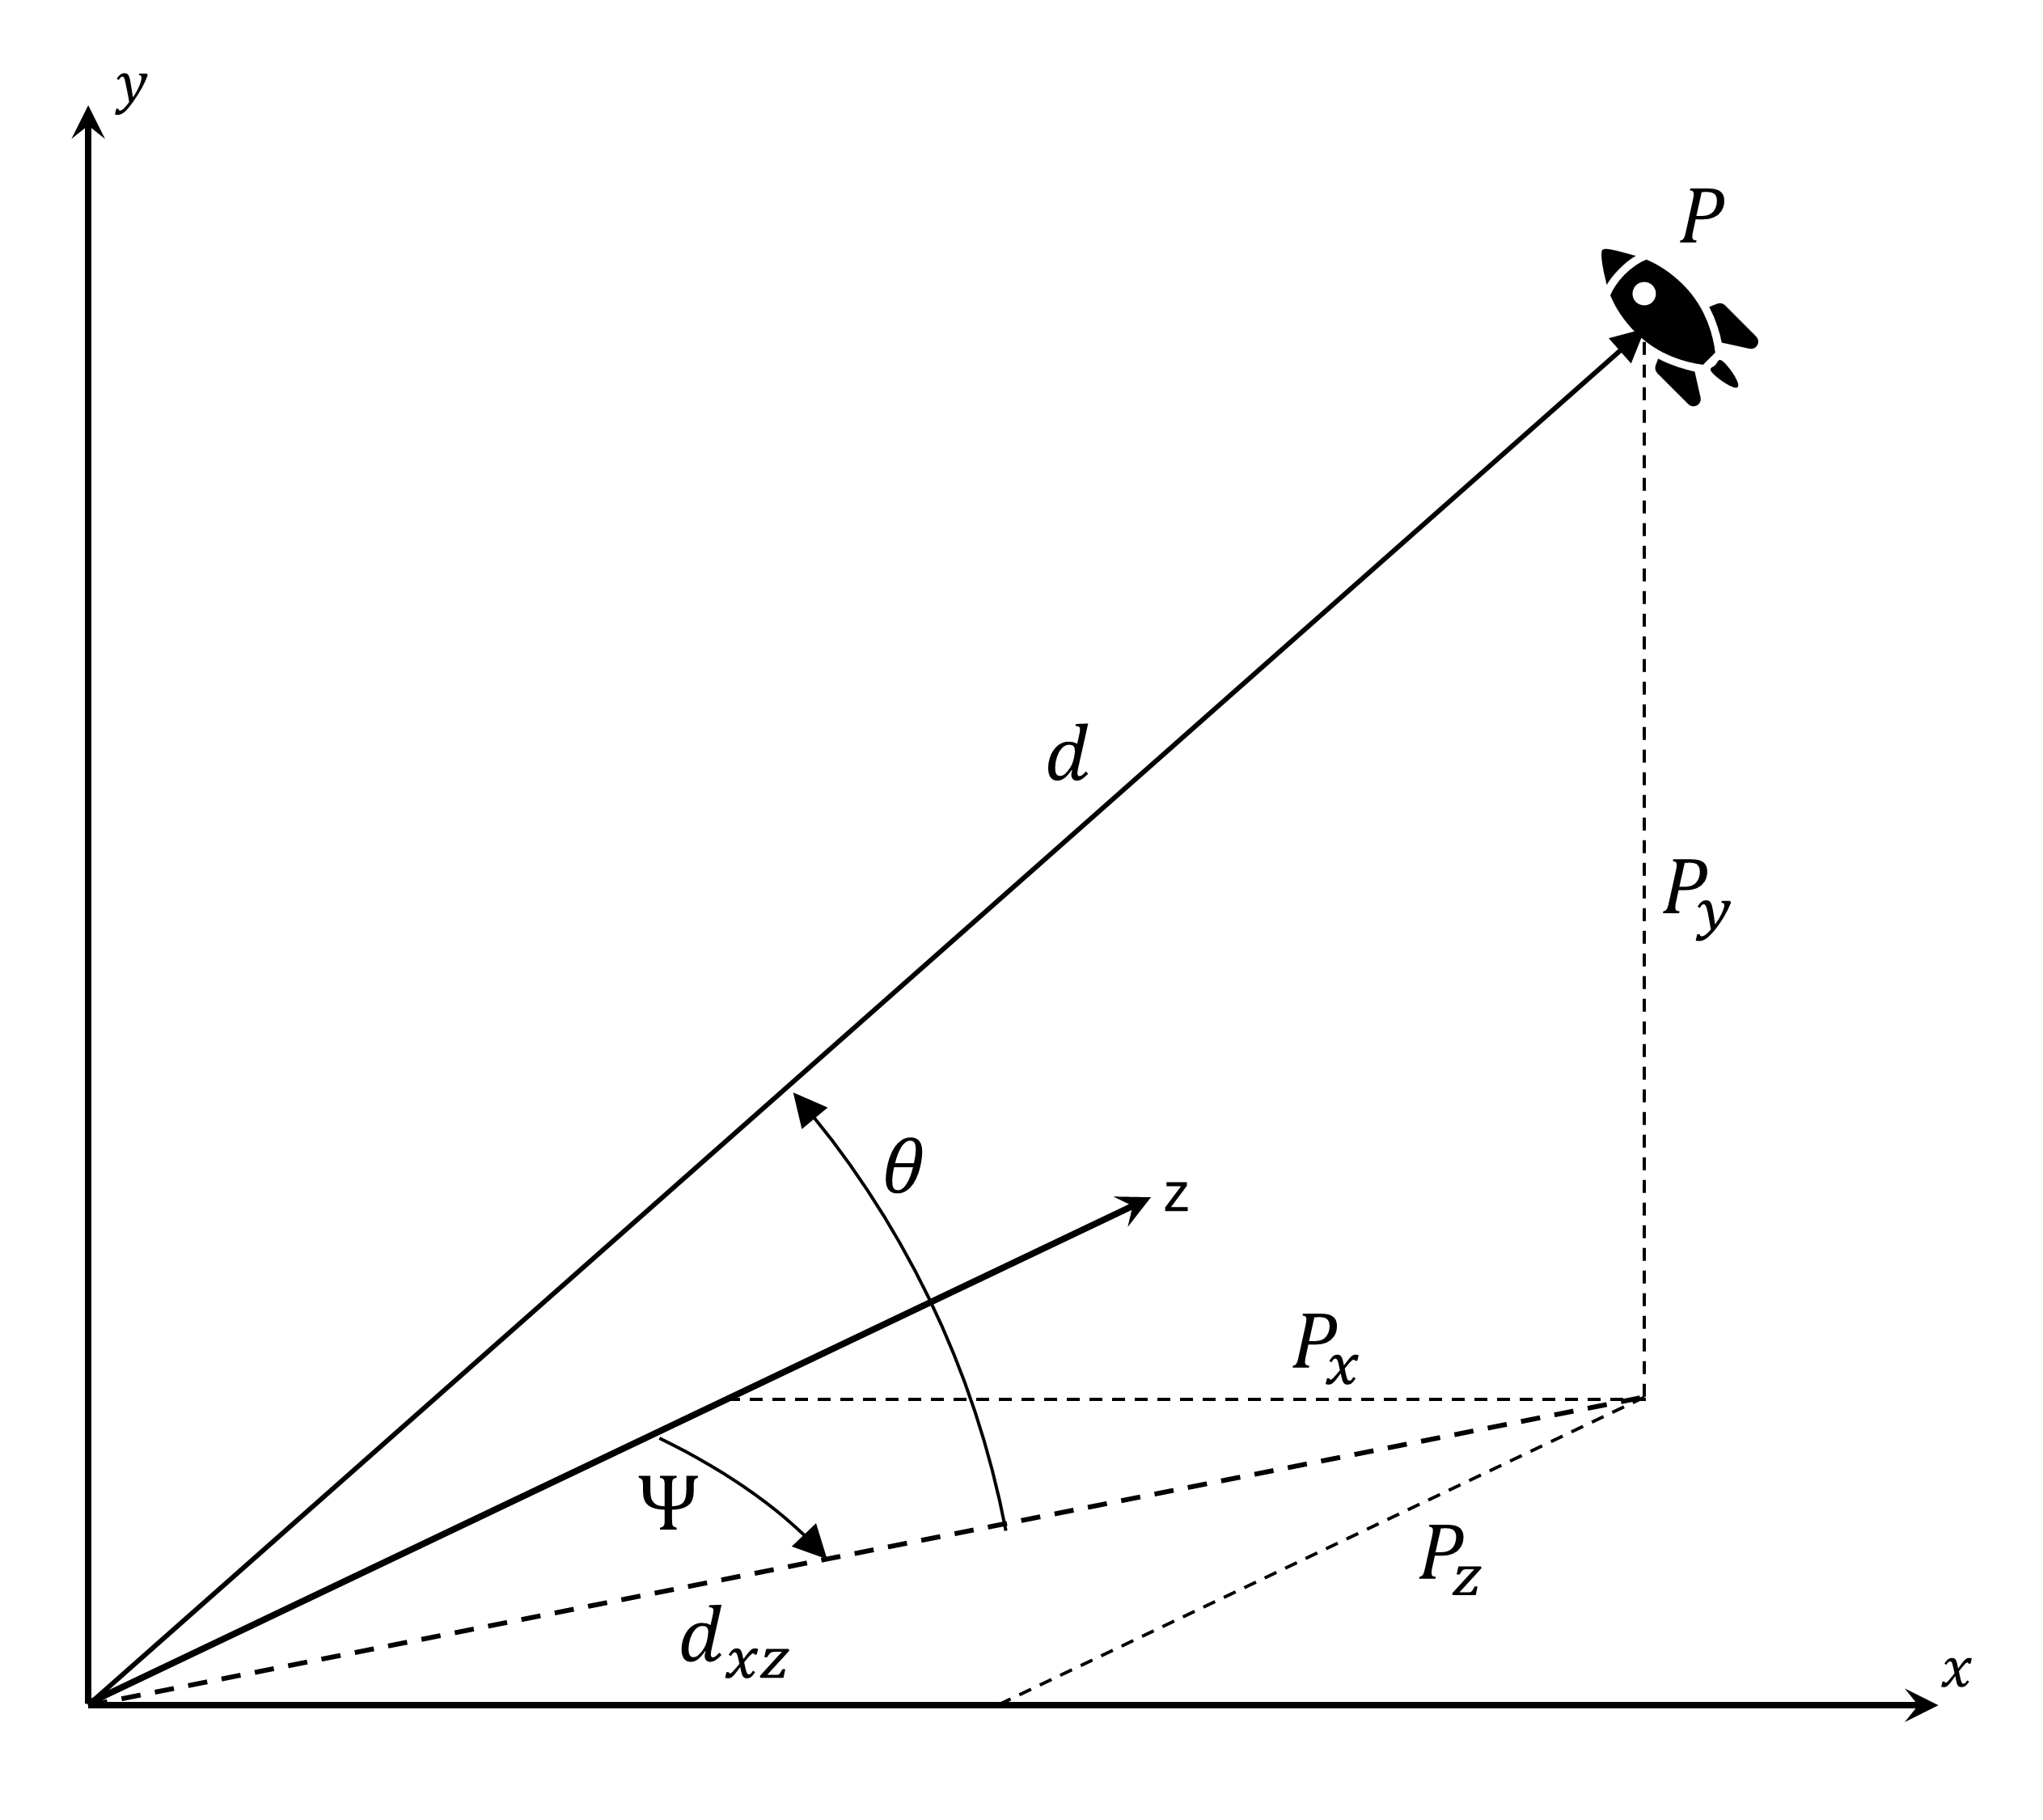
\includegraphics[width=0.8\linewidth]{AzElAtan2.png}
     \caption{Evaluation of Euler Angles using atan2}
     \label{fig:atan2}
\end{figure}
\section{Conclusion}
Quaternions are an effective and robust solution for representing orientations with three fully decoupled degrees of freedom, and they provide a convenient way to avoid the singularities associated with Euler angles. At the same time, it is important to recognize situations in which rotational motion is intentionally constrained. In these contexts, Euler angles may offer clearer semantics and more desirable behavior. Accordingly, engineers should be introduced to both representations as complementary tools, selecting the one most appropriate to the constraints and goals of the system being designed.

%%
%% The acknowledgments section is defined using the "acks" environment
%% (and NOT an unnumbered section). This ensures the proper
%% identification of the section in the article metadata, and the
%% consistent spelling of the heading.
\begin{acks}
I would like to thank my colleagues at the University of Southern California, my peers in video game development, as well as all the students who have taken classes with us over the years.
\end{acks}

%%
%% The next two lines define the bibliography style to be used, and
%% the bibliography file.
\bibliographystyle{ACM-Reference-Format}
\bibliography{Euler}


\end{document}
\endinput
%%
%% End of file `sample-sigconf.tex'.
